\documentclass{assignment}
\usepackage{hyperref}
\usepackage{listings}
\usepackage[utf8]{inputenc}
\usepackage[T1]{fontenc}
\usepackage{babel}
\usepackage{listings}
\usepackage{assignment}
\usepackage{tikz}

%\pgfplotsset{compat=1.18}


\newcommand*{\name}{Roberto Alvarado}
\newcommand*{\id}{00206411}
\newcommand*{\course}{Computer Networks}
\newcommand*{\assignment}{Homework 2}

\begin{document}
\assignmentTitle{\name}{\id}{logo.png}{\course}{\assignment}
\begin{ex}
 Let A and B be two stations attempting to transmit on an Ethernet. Each has a steady queue of
frames ready to send; A’s frames will be numbered A1, A2, and so on, and B’s similarly. Let T=
51.2µs be the exponential backoff base unit. Suppose A and B simultaneously attempt to send
frame 1, collide, and happen to choose backoff times of 0 x T and 1 x T, respectively, meaning
A wins the race and transmits A1 while B waits. At the end of this transmission, B will attempt
to retransmit B1 while A will attempt to transmit A2. These first attempts will collide, but now A
backs off for either 0 x T or 1 x T, while B backs off for time equal to one of 0 x T, . . ., 3 x T. 
\begin{itemize}
  \item Give the probability that A wins this second backoff race immediately after this first collision;
that is A’s first choice of backoff time k x 51.2 is less that B’s.
  \item Suppose A wins this second backoff race. A transmits A3, and when it is finished, A and B
collide again as A tries to transmit A4 and B tries once more to transmit B1. Give the
probability that A wins this third backoff race immediately after the first collision.
  \item Give a reasonable lower bound for the probability that A wins all the remaining backoff
races.
  \item What then happens to the frame B1?
\end{itemize}
This scenario is known as the Ethernet capture effect.
\end{ex}
\textit{ Sol. }
\begin{itemize}
  \item The idea is that A has to be smaller than B, thus as $k(A) = [0,1]$ and
    $k(B)=[0,1,2,3]$, then the case is that A is 0 and B is any other than 0 or
    A is 1 and B is either 2 or 3, thus, as we expect same probability of each
    case then
    $$P[E=A] = P[A=0,B\neq0] + P[A=1,B>1]$$
    $$P[E=A] = \frac{1}{2}*\frac{3}{4}+ \frac{1}{2}*\frac{2}{4}  $$
    $$P[E=A] = \frac{3}{8} + \frac{2}{8}  $$
    $$P[E=A] = \frac{5}{8} $$
  \item Same idea in this case $k(A) =[0,1]$ and $k(B) = [0,1,2,3,4,5,6,7]$
    $$P[E=A] = P[A=0,B\neq0] + P[A=1,B>1]$$
    $$P[E=A] = \frac{1}{2}*\frac{7}{8}+ \frac{1}{2}*\frac{6}{8}  $$
    $$P[E=A] = \frac{7}{16} + \frac{6}{16}  $$
    $$P[E=A] = \frac{13}{16} $$
  \item I think we can actually calculate for an n collision what is the
    probability for A to win, for that we can see that for $P[E=A_n]$ that is
    the probability for A to win in the n step is
    $$P[E=A_n] = \frac{2^{n}-1 + 2^{n}-2}{2^{n+1}}$$
    $$\lim_{n \to \infty} P[E=A_n] = 1$$
    For n $\in$ 3,10,20,30 we can show a table
    \begin{table}[h]
      \begin{center}
        \begin{tabular}[c]{c|c}
          \hline
          \multicolumn{1}{c|}{\textbf{n}} & 
          \multicolumn{1}{c}{\textbf{P[E=$A_n$]}} \\
          \hline
          3  &  0.95\\
          10 &  0.99926\\
          20 &  0.99999\\
          30 &  0.99999\\
          \hline
        \end{tabular}
      \caption{P for n}
    \end{center}
    \end{table}
    \\as n grows we an see this graphic 
    \begin{figure}[h]
    \begin{center}
      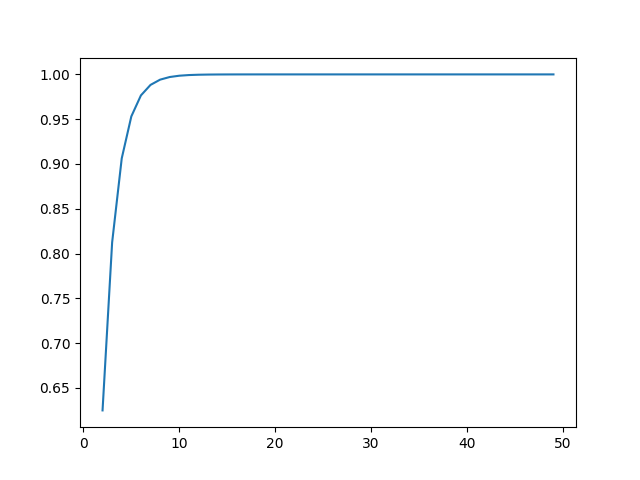
\includegraphics[scale=0.5]{figures/1.png}
    \end{center}
    \caption{Limit of P}
    \label{fig:}
    \end{figure}
    So we have to find the probability that each times it wins, thus at first we
    are going to see that we need 

    $$ P[A remaining] = \prod_{n=4}^{\infty}  \frac{2^{n}-1 + 2^{n}-2}{2^{n+1}}$$
    $$ P[A remaining] \approx 0.8245$$

    Probability drops when added the first two instances (so the important part
    is to not loose anyone)

    $$ P[A all] = \prod_{n=2}^{\infty}  \frac{2^{n}-1 + 2^{n}-2}{2^{n+1}}$$
    $$ P[A all] \approx 0.418$$

  \item If we set a limit of time that the Ethernet cable has to transmit, then
    after it passes B will drop B1, and start transmitting B2.
\end{itemize}

\newpage
\begin{ex}
  Suppose Ethernet physical addresses are chosen at random (using true random bits).
  \begin{itemize}
  \item  What is the probability that on a 1024-host network, two addresses will be the same?
  \item  What is the probability that the above event will occur on some one
    or more of $2^{20}$ networks?
  \item  What is the probability that of the $2^{30}$ hosts in all the network of (b), some pair has the
  same address?
  \end{itemize}
  Hint: Check the Birthday Problem
\end{ex}
\textit{ Sol. }

Ethernet addresses will be a 12-long char address, for simplicity is the same as
saying that the Ethernet is a 48bits char array, as a bit can only be 1 or 0,
then there exits $2^{48}$ possible addresses, but in Ethernet there are two
fixed bits, thus there is $2^{46}$ possible addresses
\begin{itemize}
  \item If there is 1024-host network then the probability is going to be
    $$P_{1024} = \frac{\sum^{1}_{i=1023} i  }{2^{46}} =
    7.4433046393096446990966796875 \times e^{-9}$$

  \item Now for $2^{20}$ then we have
    $$P_{2^{20}} = \left(1-\frac{1}{2^{46}}\right)\times \dots \times
    \left(1-\frac{2^{20}-1}{2^{46}}\right)$$
    we are going to have to find a optimization, then we can use the fact that
    $2^{20} << 2^{46}$ and then using stirling approximation 
  $$n! \approx \frac{n^n}{e^n} \sqrt{2\pi n } $$
  Making that
    $$xPy \approx y^x $$
  Then
    $$P_{2^{20}} \approx \frac{(2^{20})^2}{2*2^{46}} $$
    $$P_{2^{20}} \approx \frac{(2^{40})^2}{2^{47}} $$
    $$P_{2^{20}} \approx \frac{1}{2^{7}} = 0.007812$$
\item We could not do that for $2^{30}$ so for this we are going to do something
  sketchy, we are going to map the probability to the original birthday problem
  to our problem, as we have essentially the same distribution, we know that the
  original birthday problem and use the approximation such that
  $$P_{n} \approx 1-\prod_{i=1}^{n} e^{\frac{i}{2^{46}}}$$
  $$P_{n} \approx 1-e^{-\frac{n(n-1)}{2^{46}}}$$
  Then 
  $$P_{2^{30}} \approx 1-e^{-\frac{2^{30}(2^{30}-1)}{2^{46}}}$$
  Then
  $$P_{2^{30}} \approx 1-e^{-\frac{2^{60}}{2^{46}}}$$
  $$P_{2^{30}} \approx 1-e^{2^{14}}$$
  $$P_{2^{30}} \approx 1$$
\end{itemize}
\newpage
\begin{ex}
Why might a mesh topology be superior to a base station topology for communications in a
natural disaster?
\end{ex}
\textit{ Sol. }

First answering the question directly to a natural disaster. In this event there
is a high likelihood that one of the servers, routers, devices will be damage,
so in a mesh topology as there is a lot of redundancy of connections then the
whole network won't stop working as it has a lot of ways to distribute it self
and not be disrupted by a damaged node.
So specifically, if one of the nodes is damaged in natural disaster then the
network can find ways to reroute the data and manage the problematic node.

Another possible advantage is that as it is more flexible then we can add more
nodes in order to manage the resolution of the problem


\newpage
\begin{ex}
Suppose an IP packet is fragmented into 10 fragments, each with a 1\% (independent)
probability of loss. To a reasonable approximation, this means there is a 10\% chance of losing
the whole packet due to loss of a fragment. What is the probability of net loss of the whole
packet if the packet is transmitted twice
\begin{itemize}
\item Assuming all fragments received must have been part of the same transmission?
\item Assuming any given fragment may have been part of either transmission?
\item Explain how use of the ident field might be applicable here
\end{itemize}
\end{ex}
\begin{itemize}
  \item We can see that there is a 99\% probability that a package will get to
    it's intended destination, so let's see that there are 10 packages thus the
    probability of a net loss then is 
    $$1-0.99^{10} = 0.95617\%$$
    This is for a single fragmented fragment, as we want send two times in the
    same transmission, we have to find the probability for it to happen twice
    $$ (0.95617\%)^2 = 0.00914\%$$
  \item Now as we don't have way to separated between transmission, then the
    probability for a package loss is $0.01^2 = 0.0001$ so the probability that
    for a single fragment to not fail is going to be $1-0.0001$, thus
    for fragments the probability to be a loss is going to be
    $$1-(1-0.001)^{10} = 0.00992\%$$
  \item in this case we can see that if we do not identify between the two
    packages then is going to be a higher probability of a net loss, thus with
    the identification field will help us reduce the probability of a net loss
    if we use this technique
\end{itemize}

\newpage
\begin{ex}
  For the network given in the figure below, give the datagram forwarding table for each node.
The links are labeled with relative costs; your tables should forward each packet via the lowestcost path to its destination

\end{ex}

\begin{figure}[h]
  \begin{center}
    
  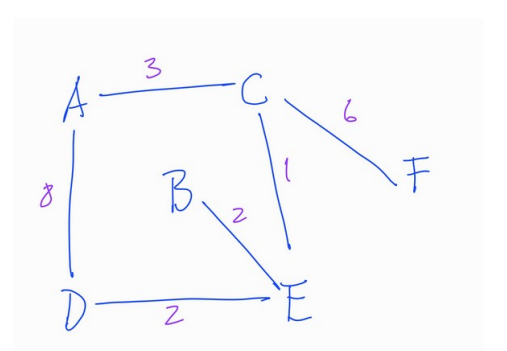
\includegraphics[scale=0.5]{figures/2.png}
\caption{Problem}
  \end{center}
\end{figure}
\textit{ Sol. }
\begin{table}[h]
\centering
\begin{tabular}{|c|c|} \hline
Destination  &  Next Hop \\ \hline
B  &  C\\
C  &  C\\
D  &  C\\
E  &  C\\
F  &  C\\ \hline
% Insert content for tables 1 and 2 here
\end{tabular}
\vspace{0.5cm}
\begin{tabular}{|c|c|} \hline
Destination  &  Next Hop \\ \hline
A&  E\\
C&  E\\
D&  E\\
E&  E\\
F&  E\\ \hline
% Insert content for tables 1 and 2 here
% Insert content for tables 3 and 4 here
\end{tabular}
\vspace{0.5cm}
\begin{tabular}{|c|c|} \hline
Destination  &  Next Hop \\ \hline
A&  A\\
B&  E\\
D&  E\\
E&  E\\
F&  F\\ \hline
% Insert content for tables 1 and 2 here
% Insert content for tables 5 and 6 here
\end{tabular}
\begin{tabular}{|c|c|} \hline
Destination  &  Next Hop \\ \hline
A&  E\\
B&  E\\
C&  E\\
E&  E\\
F&  E\\ \hline
% Insert content for tables 1 and 2 here
% Insert content for tables 3 and 4 here
\end{tabular}
\begin{tabular}{|c|c|} \hline
Destination  &  Next Hop \\ \hline
A&  C\\
B&  B\\
C&  C\\
D&  D\\
F&  C\\ \hline
% Insert content for tables 1 and 2 here
% Insert content for tables 3 and 4 here
\end{tabular}
\begin{tabular}{|c|c|} \hline
Destination  &  Next Hop \\ \hline
A&  C\\
B&  C\\
C&  C\\
D&  C\\
E&  C\\ \hline
% Insert content for tables 1 and 2 here
% Insert content for tables 3 and 4 here
\end{tabular}
\caption{Datagram}
\label{tab:six_tables}
\end{table}
Respectively for each of the node that is missing for the table
\newpage
\begin{ex}
  Given the extended LAN shown in the figure below, indicate which posts are not selected by
the spanning tree algorithm
\end{ex}
\begin{figure}[h]
\begin{center}
  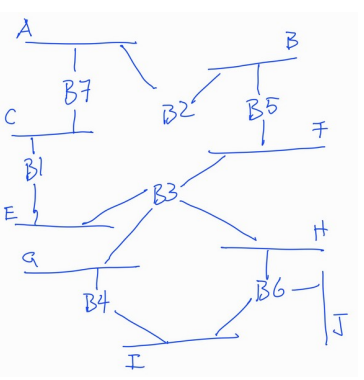
\includegraphics[scale=0.5]{figures/2_000.png}
\end{center}
\caption{Problem}
\label{fig:probelm}
\end{figure}
Solved using algorithm made in \url{https://github.com/Robdres/spanningTree}\\
If we take that the root is going to be B1 then, we have that the post that are
not selected are
\begin{itemize}
  \item B
  \item D
  \item F
  \item I 
\end{itemize}
But we can also make it for B3 that gives better results

\begin{itemize}
  \item A
  \item I
\end{itemize} 
\newpage
\begin{ex}
Use the Unix tool traceroute (Windows tracert) to determine how many hops it is from your
host to other hosts in the internet (usfq.edu.ec, google.com, amazon.com, etc). How many
routers do you traverse to get out of your local site? Read the documentation of this tool, and
explain how it is implemented. 
\end{ex}

First let's test for google.com that is 12 nodes
\begin{figure}[h]
\begin{center}
  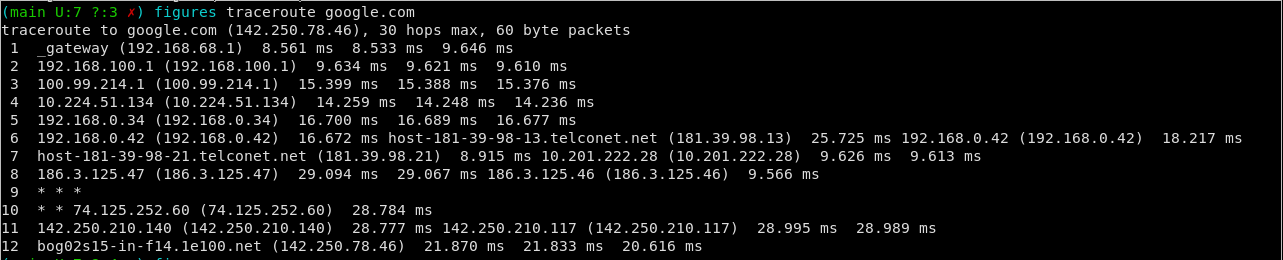
\includegraphics[scale=0.3]{figures/2_001.png}
\end{center}
\caption{Google.com traceroute}
\end{figure}

For usfq.edu.ec that is 30 nodes
\begin{figure}[h]
\begin{center}
  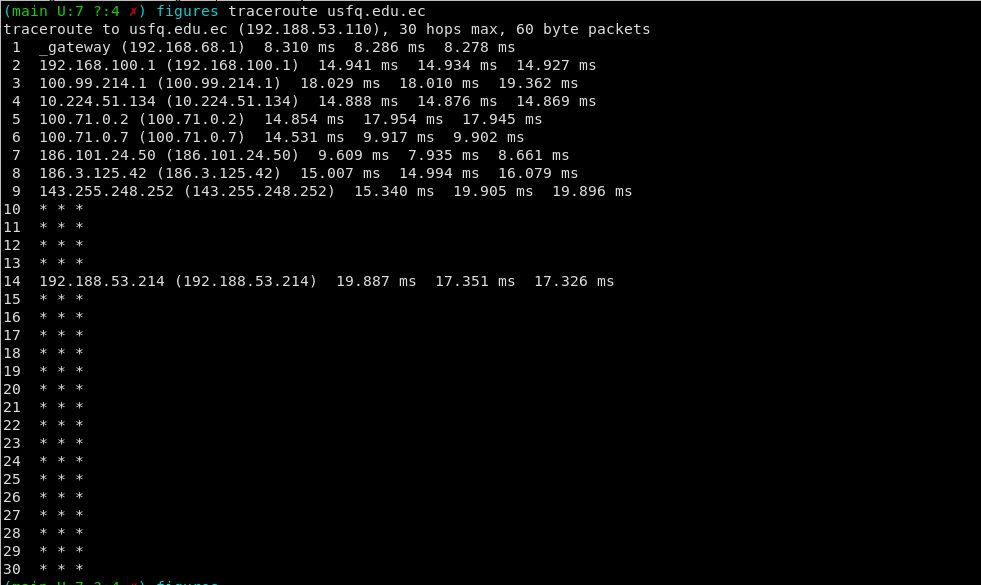
\includegraphics[scale=0.3]{figures/2_002.png}
\end{center}
\caption{Usfq.edu.ec traceroute}
\end{figure}

For facebook.com that is 11 nodes!
\begin{figure}[h]
\begin{center}
  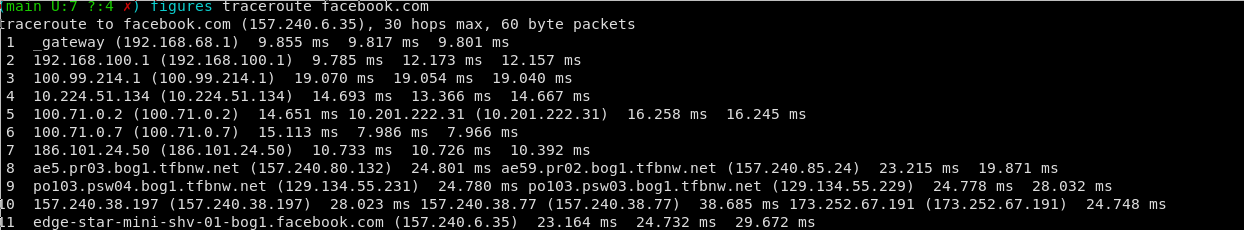
\includegraphics[scale=0.3]{figures/2_004.png}
\end{center}
\caption{facebook.com traceroute}
\end{figure}
\newpage
For amazon.com that is 30 routers
\begin{figure}[h]
\begin{center}
  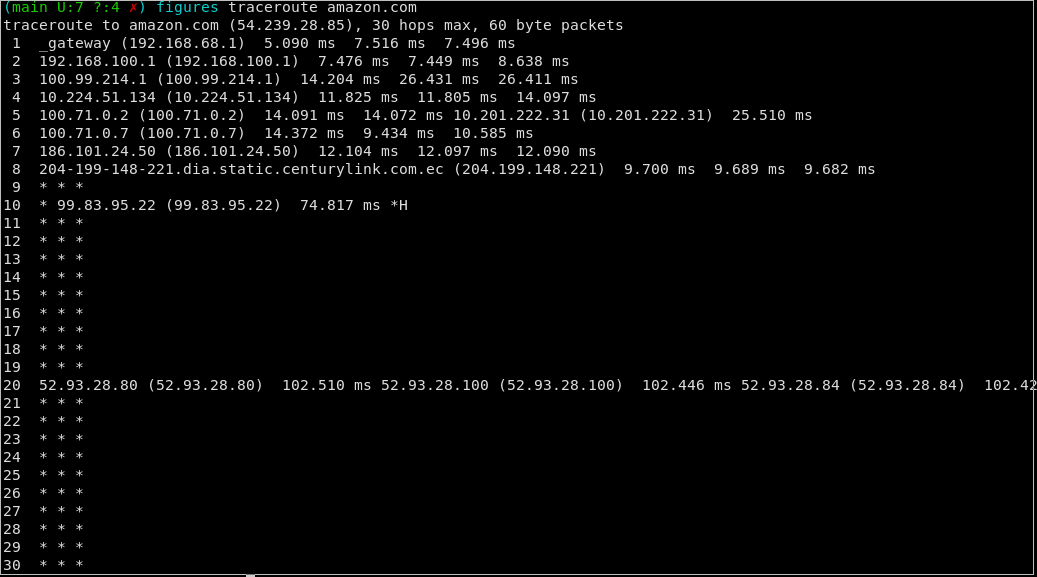
\includegraphics[scale=0.3]{figures/2_003.png}
\end{center}
\caption{amazon.com traceroute}
\end{figure}

The command $man~traceroute$ specifies how this program works

\begin{lstlisting}[language=bash]
  traceroute  tracks  the  route packets taken from an IP network on their way
  to a given host. It utilizes the IP protocols time to live
  (TTL) field and attempts to elicit an ICMP TIME_EXCEEDED response from
  each gateway along the path to the host.
\end{lstlisting}

     \vspace{1cm}
This programs permits to make a tracerouting using IPv6 protocol
\begin{lstlisting}[language=bash]
-4, -6 Explicitly force IPv4 or IPv6 tracerouting. By default, the program will try to resolve the name given, and choose the  appropriate protocol automatically. If resolving a host name returns both IPv4 and IPv6 addresses, traceroute will use IPv4.
\end{lstlisting}

\vspace{1cm}
For example we can make a traceroute using IPv6 protocol with pages
that handles it, for example, google.com that only have 1 router that uses IPv6
\begin{figure}[h]
\begin{center}
  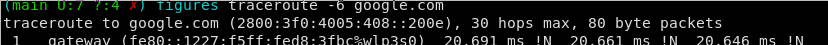
\includegraphics[scale=0.5]{figures/2_005.png}
\end{center}
\label{fig:Google IPv6 tracerouting}
\end{figure}

Finally we can setup our own starting route with $-s$

\begin{lstlisting}[language=bash]
-s source\_addr, --source=source\_addr
      Chooses  an  alternative source address. Note that you must select the address of one of the interfaces.  By default, the address
      of the outgoing interface is used.
\end{lstlisting}
\newpage
\begin{ex}
  An ISP with a class B address is working with a new company to allocate it a portion of
address space based on CIDR. The new company needs IP addresses for machines in three
divisions of its corporate network: Engineering, Marketing, and Sales. These divisions plan to
grow as follows: Engineering has 5 machines as of the start of year 1 and intends to add 1
machine every week; Marketing will never need more than 16 machines; and Sales needs 1
machine for every two clients. As of the start of year 1, the company has no clients, but the
sales model indicates that by the start of year 2, the company will have six clients and each
week thereafter gets one new client with probability 60\%, loses one client with
probability 20\%,
or maintains the same number with probability 20\%.
\begin{itemize}
\item What address range would be required to support the company’s growth plans for at least
seven years if marketing uses all 16 of its addresses and the sales and engineering plans
behave as expected?
\item How long would this address assignment last? At the time when the company runs out of
address space, how would the addresses be assigned to the three groups?
\item If CIDR addressing were not available for the 7-year plan, what options would the new
company have in terms of getting address space?
\end{itemize}
\end{ex}
\begin{itemize}
  \item For the first question we get have to get the number of ip addresses
    needed for the first 7 years
    $$IP\_Addresses = Engineering + Marketing + Sales$$
    $$Engineering = 5 + 1*7*52 = 369$$
    $$Marketing = 16$$
    For sales we are going to use the expected values
    $$Sales =( 6 + 0.6*6*52 - 0.2*6*52 )/ 2= 130 /2 = 65 $$
    Thus 
    $$IP\_Addresses = 440$$
    So we need a subnet for the immediately superior power of 2, meaning $2^9=
    512$ thus the subnet mask that we will need, based on IPv4 is going to be $32-9 =
    23$ for IPv6 is going to be $128-9=119$
  \item It will last for 7 years as it was stated in a), and each of the
    departments will have
    \begin{table}[h]
      \begin{center}
        \begin{tabular}[c]{l|l}
          \hline
          \multicolumn{1}{c|}{\textbf{Department}} & 
          \multicolumn{1}{c}{\textbf{addresses}} \\
          \hline
          Engineering& 369 \\
          Marketing & 16 \\
          \hline
          Sales & 65 \\
        \end{tabular}
      \caption{Ip addresses distribution}
      \end{center}
    \end{table}
  \newpage
  \item There are different options
    \begin{itemize}
      \item First it can use private addressing inside its company and using
        Network \\Address Translation, that could help the company to share a
        single multiple IP address 
      \item The other thing can be to apply to multiple class C IP addresses,
        one is not enough
          
    \end{itemize}
    
\end{itemize}
\end{document}
